\documentclass[aspectratio=169,xcolor=dvipsnames]{beamer}
\usetheme{metropolis}

\usepackage{hyperref}
\usepackage{graphicx}
\usepackage{booktabs} % Allows the use of \toprule, \midrule and \bottomrule in tables
\usepackage{amsmath}
\usepackage{tabularx}
%----------------------------------------------------------------------------------------
%    TITLE PAGE
%----------------------------------------------------------------------------------------

\title{Explaining the Diversification Discount}
\subtitle{JOSE MANUEL CAMPA and SIMI KEDIA}

\author{Discussant: Ang Zhang}


\date{\today} % Date, can be changed to a custom date

%----------------------------------------------------------------------------------------
%    PRESENTATION SLIDES
%----------------------------------------------------------------------------------------

\begin{document}

\begin{frame}
    % Print the title page as the first slide
    \titlepage
\end{frame}

\begin{frame}{Overview}
    % Throughout your presentation, if you choose to use \section{} and \subsection{} commands, these will automatically be printed on this slide as an overview of your presentation
    \tableofcontents
\end{frame}

%------------------------------------------------
\section{Diversification at a glance}
%------------------------------------------------

\begin{frame}{Gains and losses of Diversification}
    \begin{block}{Benefits}
        \begin{itemize}
            \item Managerial economic of scale
            \item Internal capital market
            \item Internalize market failure / reduction of adverse selection
            \item Firm-specific asset exploitation in other industry
        \end{itemize}

    \end{block}
    \begin{block}{Costs}
        \begin{itemize}
            \item Inefficiency in resource allocation
            \item Manager rent seeking internally / value-destroying investment
            \item Internal incentives
        \end{itemize}

    \end{block}
\end{frame}

\begin{frame}
    \Huge{\centerline{\textbf{Endogeneity}}}
\end{frame}

\begin{frame}{Measurement of Diversification}
    \begin{block}{Imputed value}
        $Imputed value = \sum_{i=1}^{N} Sales_i \times Sales/Asset Multiplier$
    \end{block}
    \begin{block}{excess value}
        $\text{Excess Value} = log(\frac{Market Value}{Imputed Value})$
    \end{block}
    \begin{block}{Industry definition}
        Narrowest SIC with at least 5 firms. (4-digit and 3-digits)
    \end{block}
\end{frame}

\begin{frame}
    \Large{\centerline{\textbf{Fun fact: this study used "Tape" version of Compustat}}}
\end{frame}


\begin{frame}{Measurement of Diversification}
    \begin{figure}
        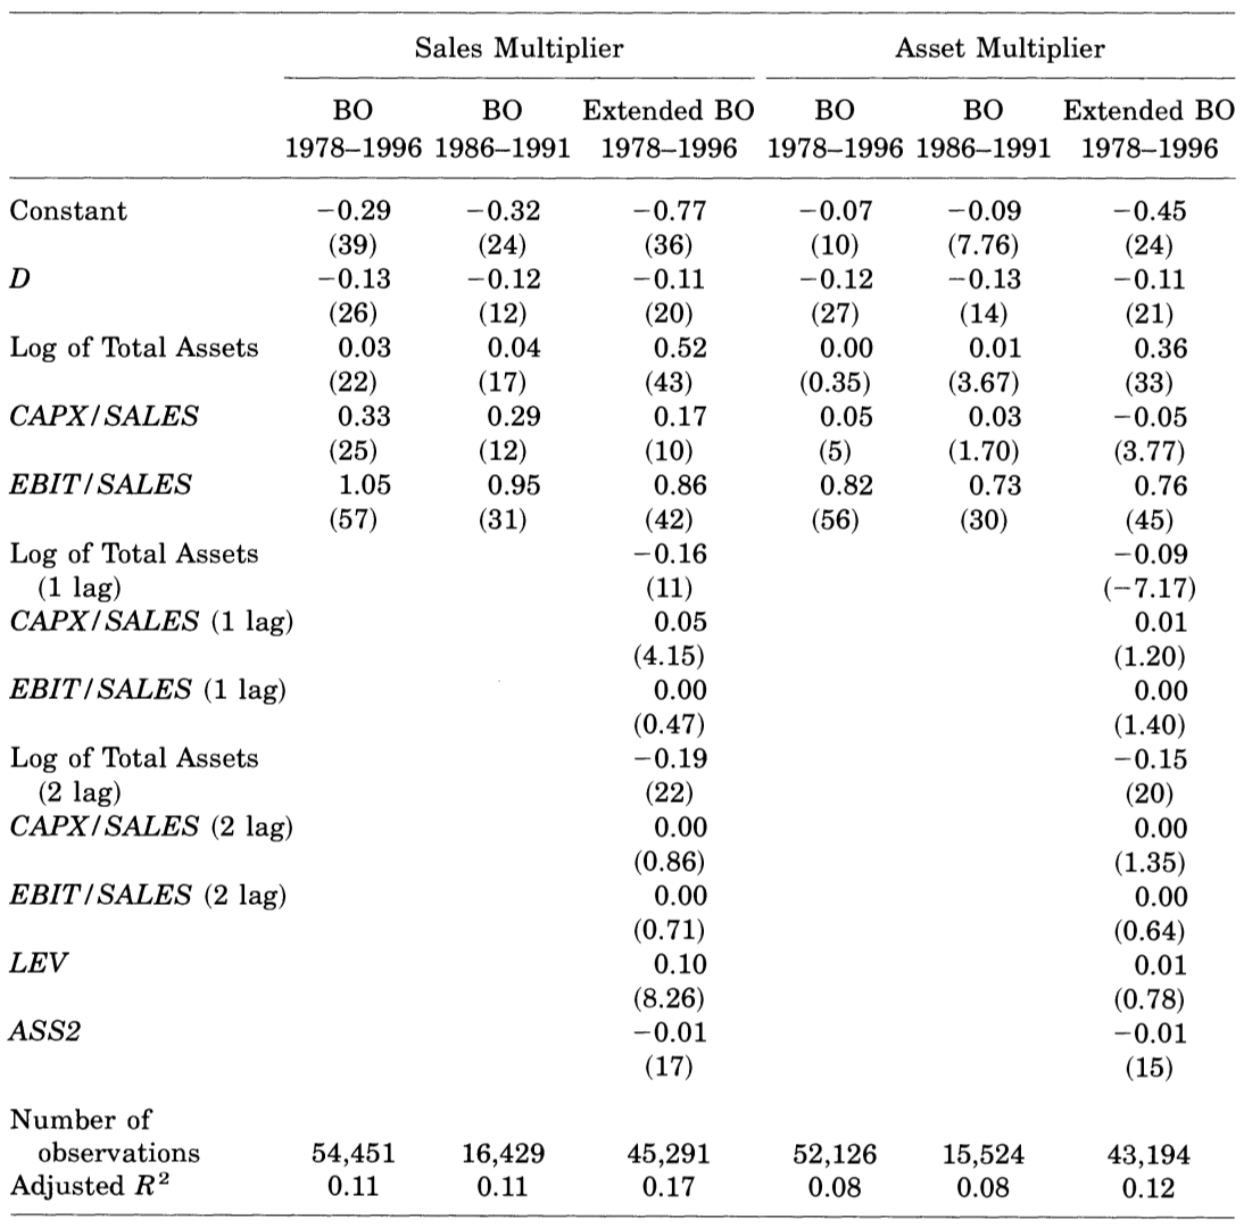
\includegraphics[width=0.5\linewidth]{figures/table1.png}
        \caption{Diversification Discount}
    \end{figure}
\end{frame}

\begin{frame}{Firm distribution}
    \begin{figure}
        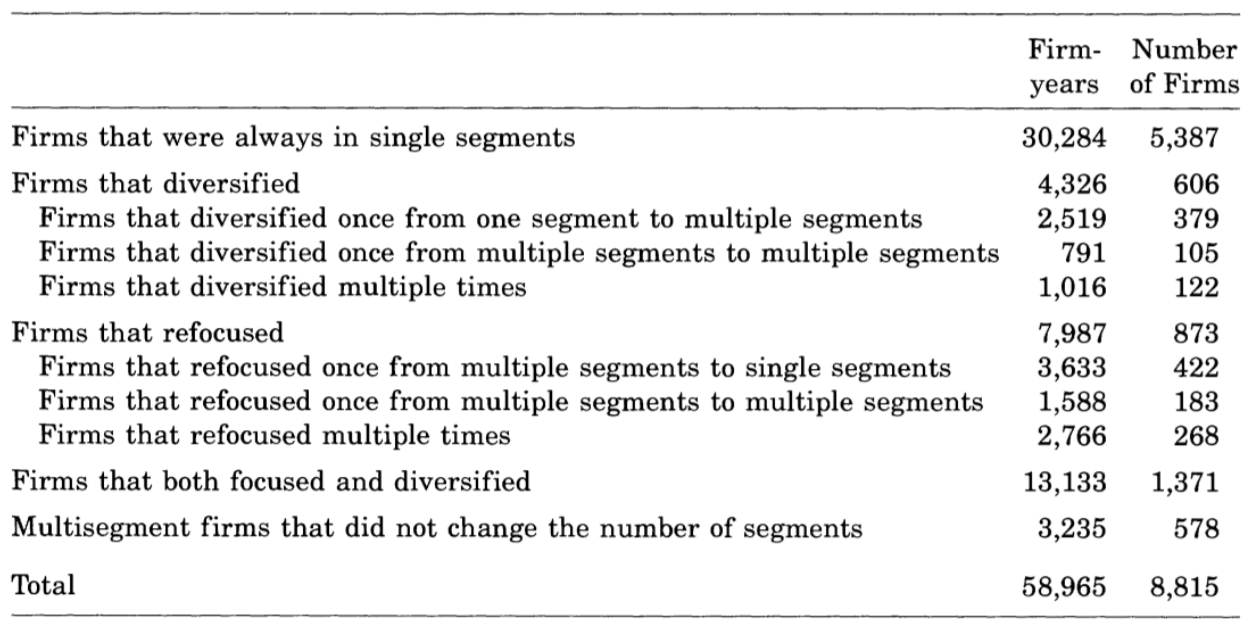
\includegraphics[width=0.8\linewidth]{figures/table2.png}
        \caption{Diversification profiles}
    \end{figure}
\end{frame}

\begin{frame}{Are conglomerates different?}
    \begin{figure}
        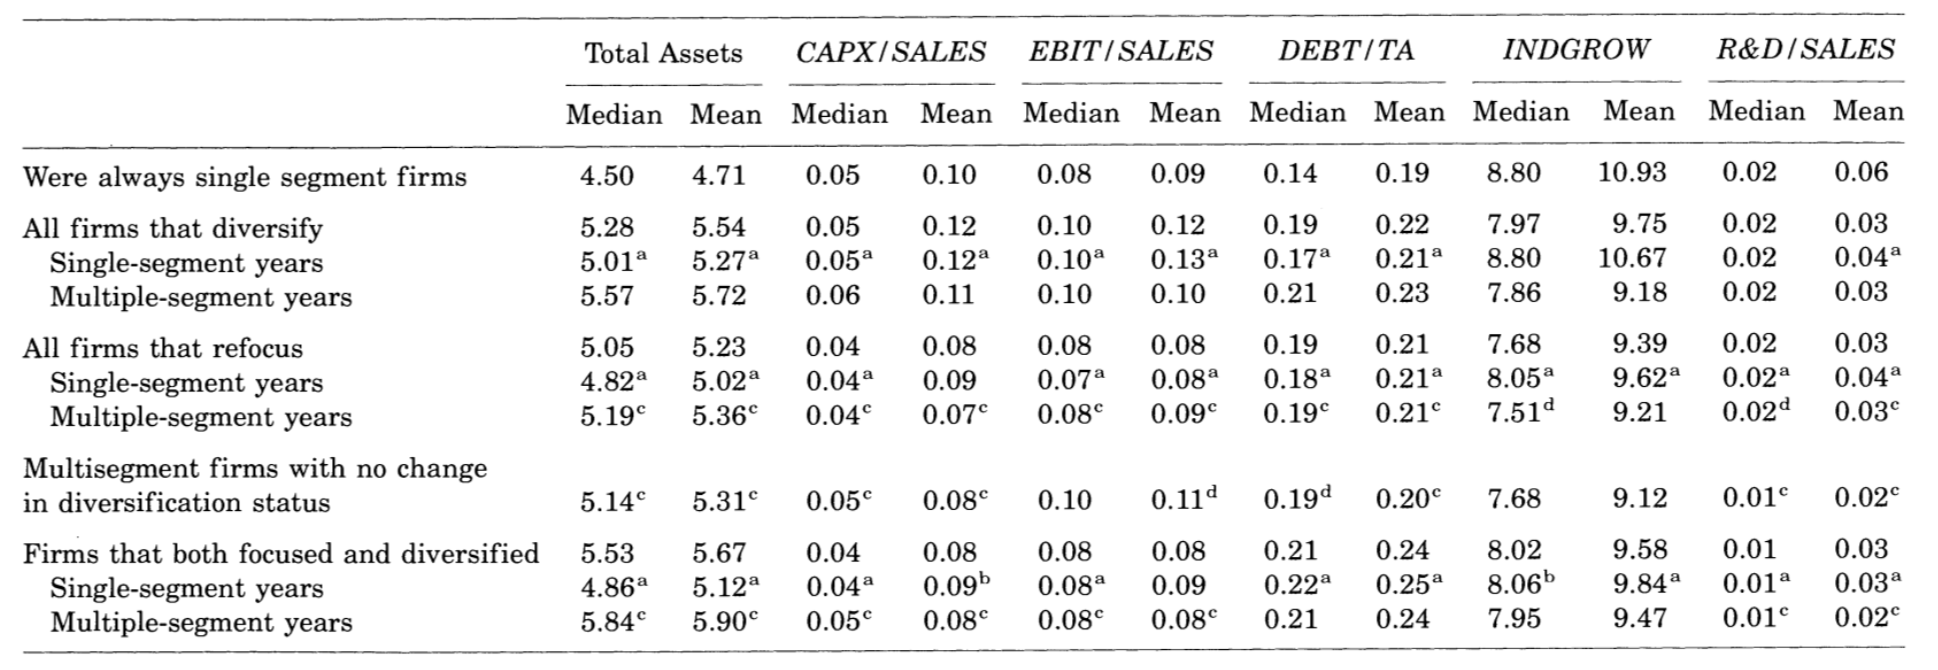
\includegraphics[width=1\linewidth]{figures/table3.png}
        \caption{Firm characteristics vs Diversification profile}
    \end{figure}
\end{frame}

\begin{frame}{Industry composition vs excess value}
    \begin{figure}
        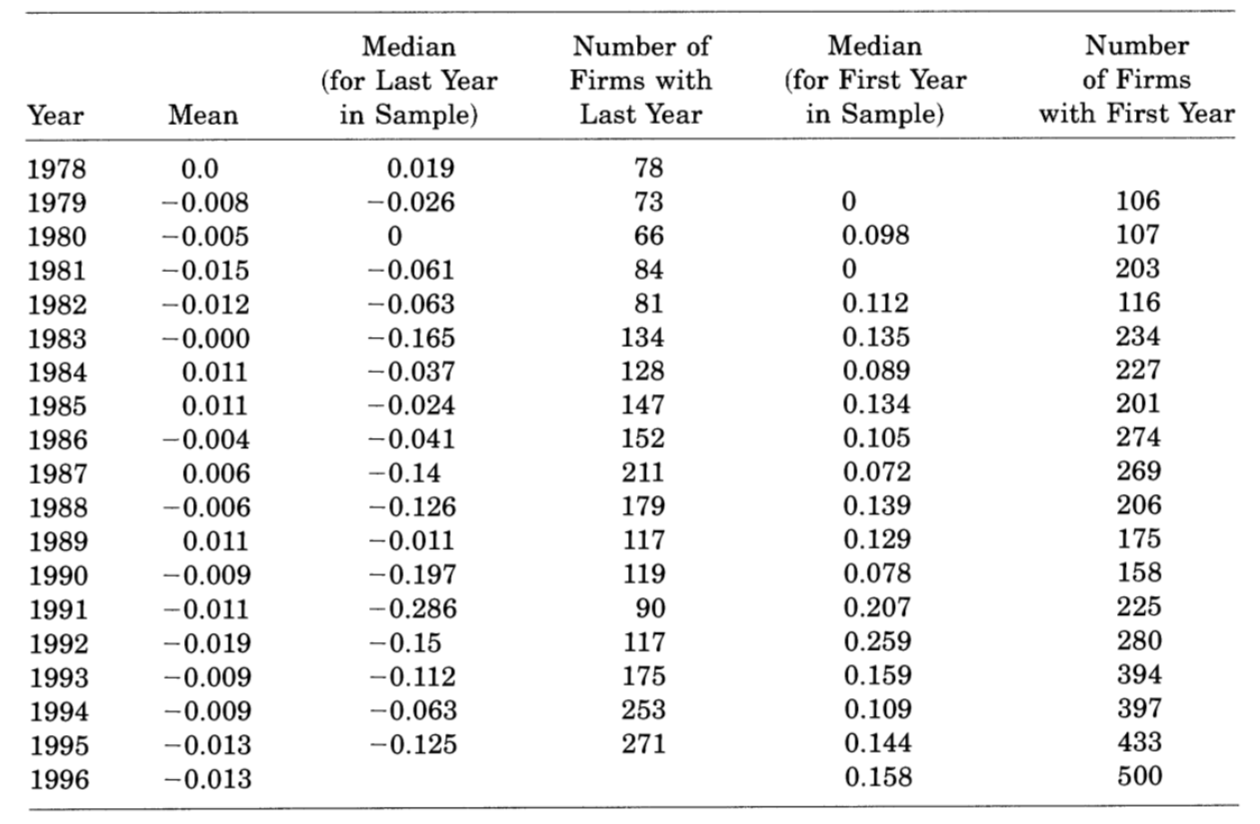
\includegraphics[width=0.7\linewidth]{figures/table4.png}
        \caption{Industry composition vs excess value}
    \end{figure}
\end{frame}

\begin{frame}{Distribution of exiting firms}
    \begin{figure}
        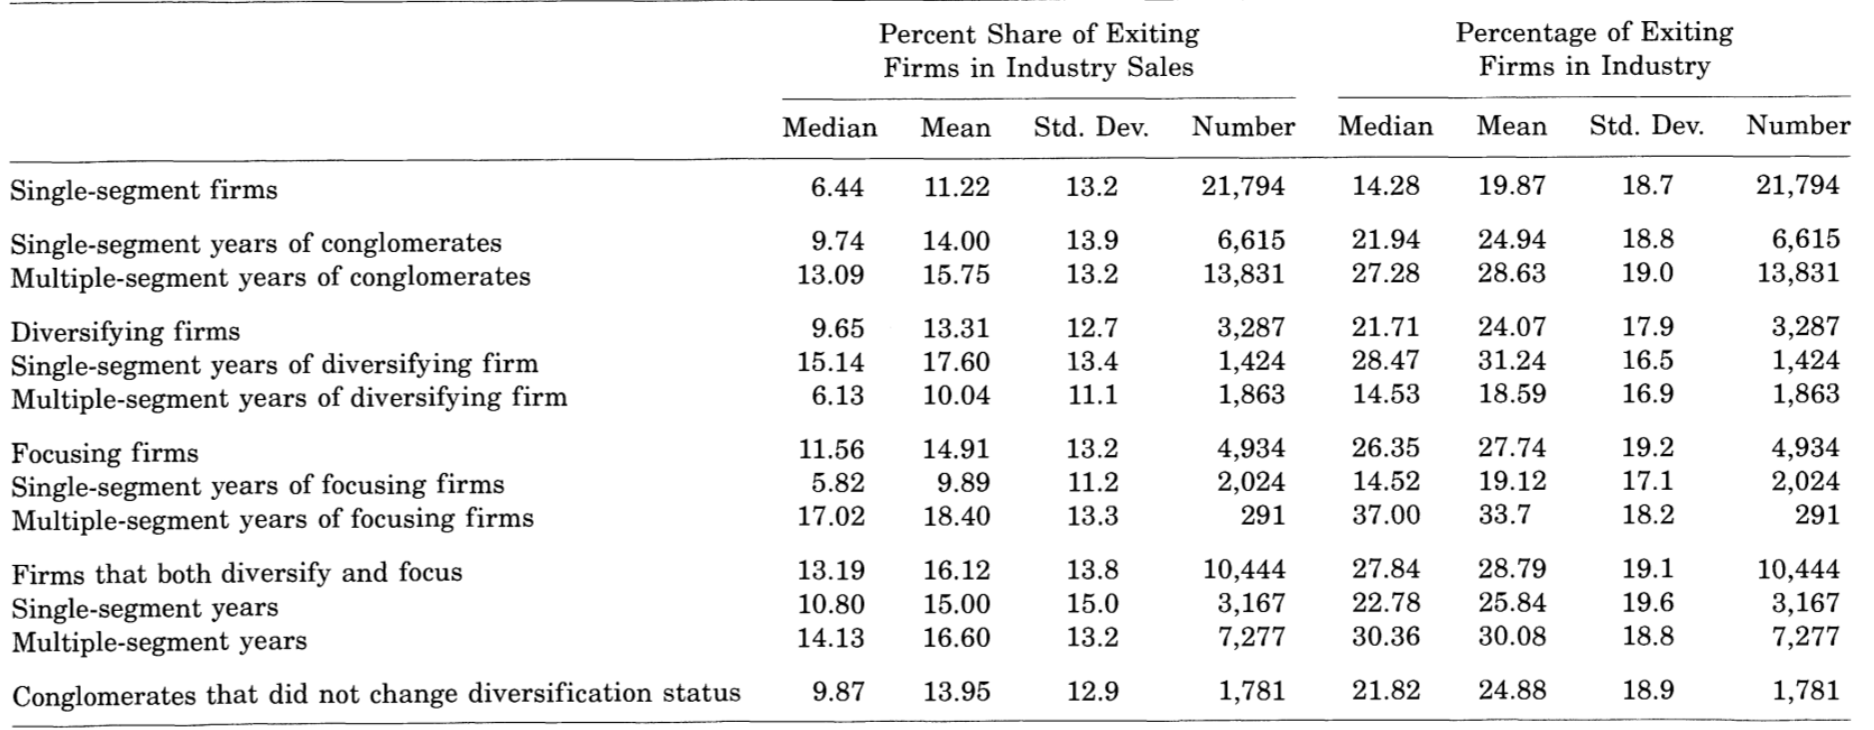
\includegraphics[width=1\linewidth]{figures/table5.png}
        \caption{Distribution of exiting firms}
    \end{figure}
\end{frame}

\begin{frame}{Existing firms and excess value}
    \begin{figure}
        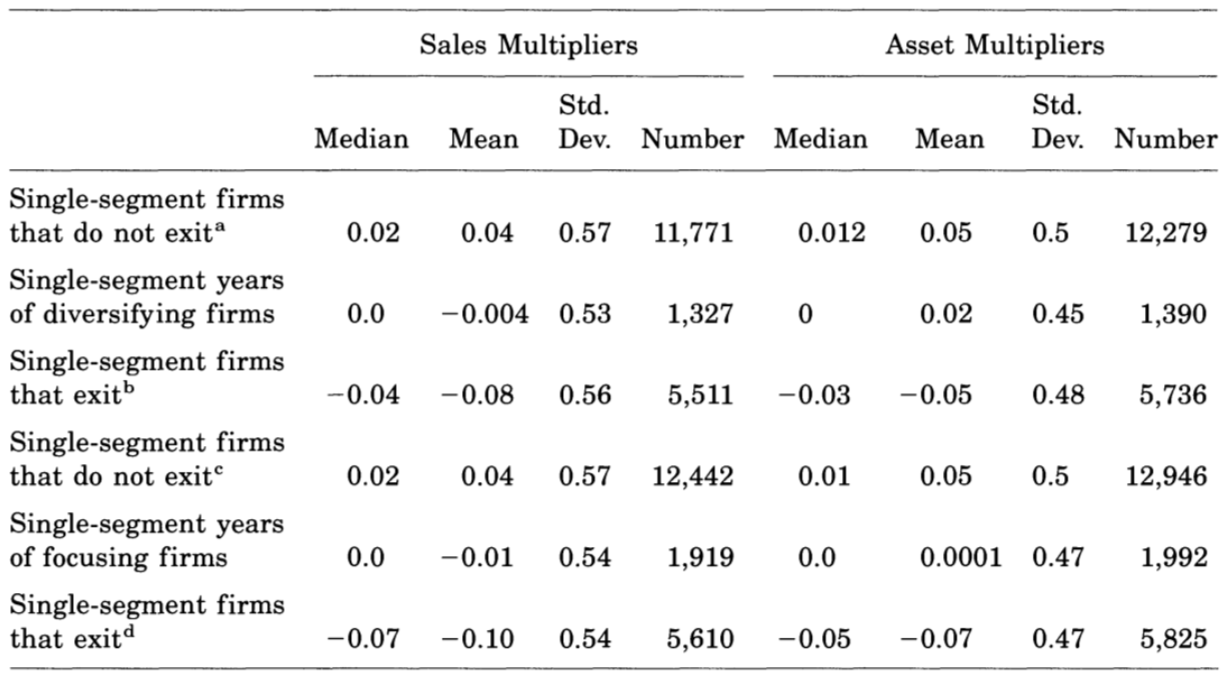
\includegraphics[width=0.85\linewidth]{figures/table6.png}
        \caption{Diversification firms vs exiting firms}
    \end{figure}
\end{frame}

\begin{frame}{What we have so far}
    \begin{block}{up to this point:}
        \begin{itemize}
            \item Conglomerates are different
            \item Diversification decision is not random
            \item Need something to control for endogeneity
        \end{itemize}
    \end{block}
\end{frame}

\section{Methodologies}

\begin{frame}{Firm value selection model}
    \begin{block}{relative firm value:}
        \begin{equation}
            V_{i,t} = \delta_0 + \delta_1 X_{i ,t} + \delta_2 D_{i,t} + \epsilon_{i,t}
        \end{equation}
    \end{block}
    \begin{block}{Diversification dummy D}
        \begin{equation}
            D^*_{i,t}  = \beta Z_{i, t} + \mu_{i,t}
        \end{equation}
        Latent variable $D^*_{i,t}$.
        \begin{equation}
            D_{i,t} = 1 \text{ if } D^*_{i,t} > 0
        \end{equation}
        \begin{equation}
            D_{i,t} = 0 \text{ if } D^*_{i,t} \leq 0
        \end{equation}
    \end{block}
    \begin{block}{Problem arises when:}
        \begin{itemize}
            \item $mu_{i,t}$ is correlated with $\epsilon_{i,t}$
            \item Unobserved heterogeneity
        \end{itemize}
    \end{block}
\end{frame}

\begin{frame}{Methodologies}
    \begin{block}{Firm fixed effect}
        assumption: unobserved heterogeneity is time-invariant

    \end{block}

    \begin{block}{IV}
        Value measure relative to industry thus industry neutral.

    \end{block}
    \begin{block}{Heckman Self-selection model}


    \end{block}
\end{frame}

\begin{frame}{IV}
    \begin{block}{Industry characters}
        \begin{itemize}
            \item Industry attractiveness: PNDIV / PSDIV

        \end{itemize}

    \end{block}
    \begin{block}{Time characters}
        \begin{itemize}
            \item M\&A: MNUM (M\&A count year)
            \item MVOL: \$ value of M\&A
            \item GDP
            \item CONTRAC: business cycle

        \end{itemize}
    \end{block}

    \begin{block}{Firm characters}
        \begin{itemize}
            \item MAJOREX: dummy variable for listed firm
            \item SNP
            \item FOREIGN: MNC firms

        \end{itemize}
    \end{block}

\end{frame}

\begin{frame}{Self-selection model}
    \begin{block}{Heckman model}
        \begin{equation}
            \begin{aligned}
                E(V_{i,t} | D_{i,t} = 1) = \delta_0 + \delta_1 X_{i ,t} + \delta_2 + E(\epsilon_{i,t} | D_{i,t} = 1) \\
                E(\epsilon_{i,t} | D_{i,t} = 1) = \rho \sigma_{\epsilon} \lambda_1 (\beta Z_{i,t})
            \end{aligned}
        \end{equation}
        \begin{equation}
            \lambda_1 (\beta Z_{i,t}) = \frac{\phi(\beta Z_{i,t})}{\Phi(\beta Z_{i,t})}
        \end{equation}

        \begin{equation}
            E(V_{i,t} | D_{i,t} = 0) = \delta_0 + \delta_1 X_{i ,t} + E(\epsilon_{i,t} | D_{i,t} = 0)
        \end{equation}
        \begin{equation}
            E(\epsilon_{i,t} | D_{i,t} = 0) = \rho \sigma_{\epsilon} \lambda_2 (\beta Z_{i,t})
        \end{equation}
        \begin{equation}
            \lambda_2 (\beta Z_{i,t}) = \frac{\phi(\beta Z_{i,t})}{\Phi(\beta Z_{i,t})}
        \end{equation}
    \end{block}
\end{frame}

\begin{frame}{Self-selection model}
    \begin{block}{Biased estimator of $\delta_2$}
        \begin{equation}
            \begin{aligned}
                E(V_{i,t}| D_{i,t}=1) - E(V_{i,t}| D_{i,t}=0) & = \delta_2 + \rho \sigma_{\epsilon} \lambda_1 (\beta Z_{i,t}) - \rho \sigma_{\epsilon} \lambda_2 (\beta Z_{i,t}) \\
                                                              & = \delta_2 + \rho \sigma_{\epsilon} \frac{\phi(\beta Z_{i,t})}{\Phi(\beta Z_{i,t})(1-\Phi(\beta Z_{i,t}))}
            \end{aligned}
        \end{equation}
    \end{block}
    \begin{block}{2-step}
        \begin{equation}
            \begin{aligned}
                V_{i,t} & = \delta_0 + \delta_1 X_{i ,t} + \delta_{\lambda} [\lambda_1(\hat{\beta} Z_{i,t})D_{i,t} + \lambda_2(\hat{\beta} Z_{i,t})(1-D_{i,t})] + \eta_{i,t} \\
                        & = \delta_0 + \delta_1 X_{i, t} \delta_2 D_{i, t} + \eta_{i, t}
            \end{aligned}
        \end{equation}
        where $\delta_{\lambda} = \rho \sigma_{\epsilon}$.
    \end{block}
\end{frame}

\begin{frame}{For diversifying firms}
    \begin{figure}
        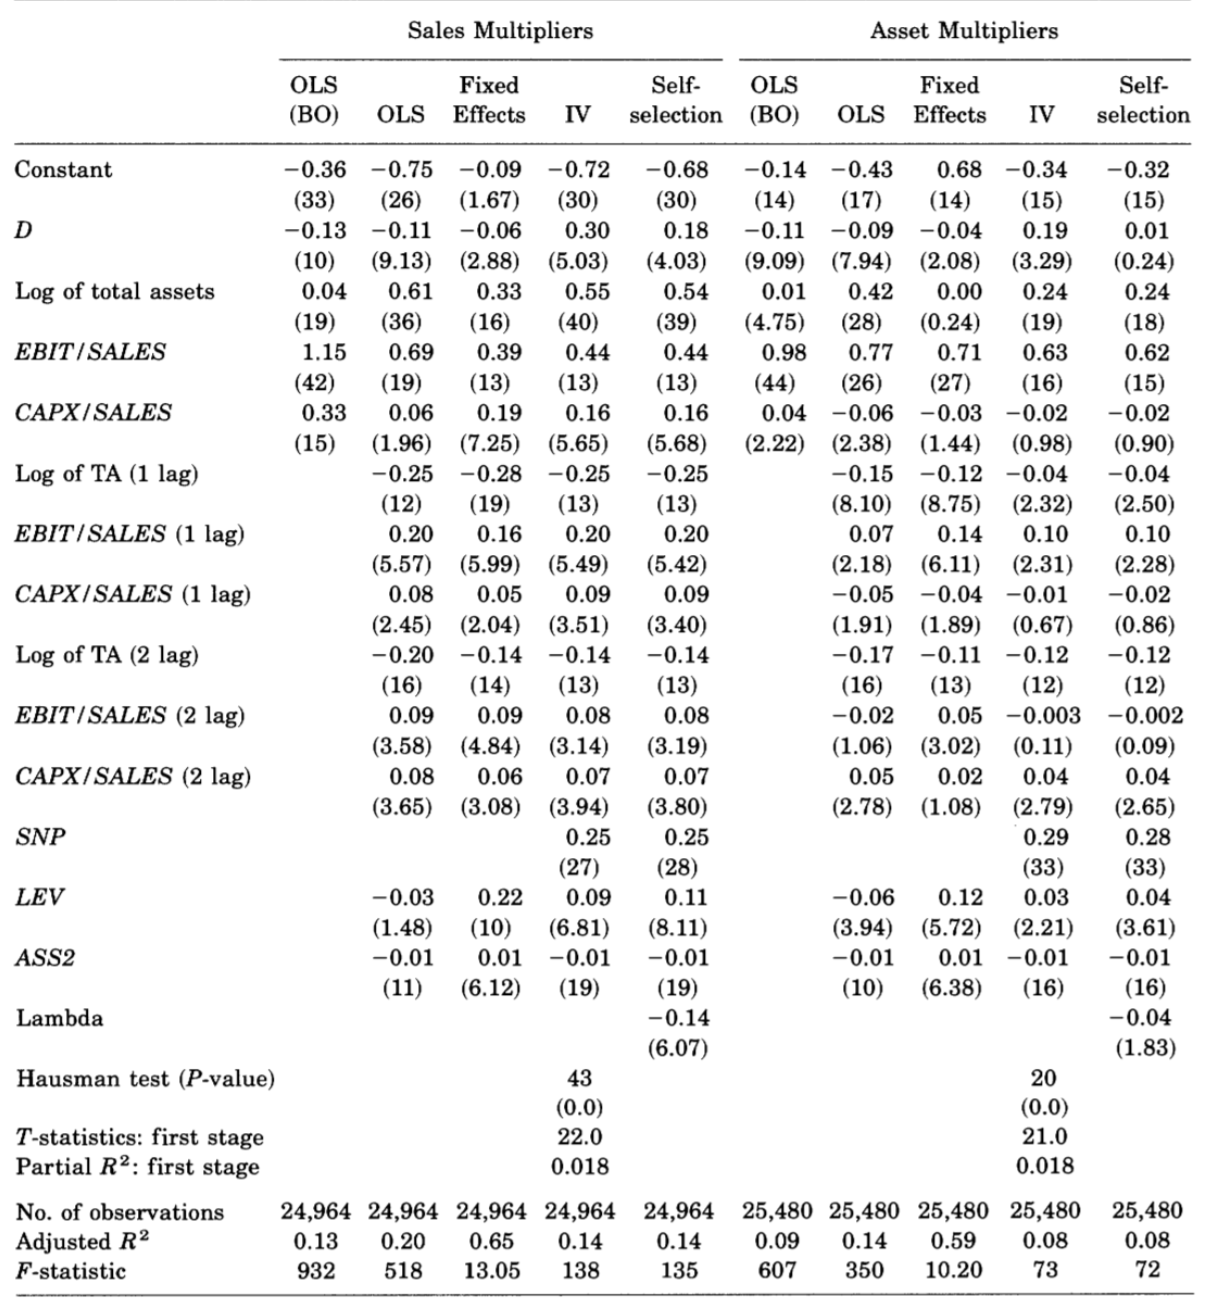
\includegraphics[width=0.5\linewidth]{figures/table7.png}
        \caption{}
    \end{figure}
\end{frame}

\begin{frame}{Probit estimates for diversitying firms}
    \begin{figure}
        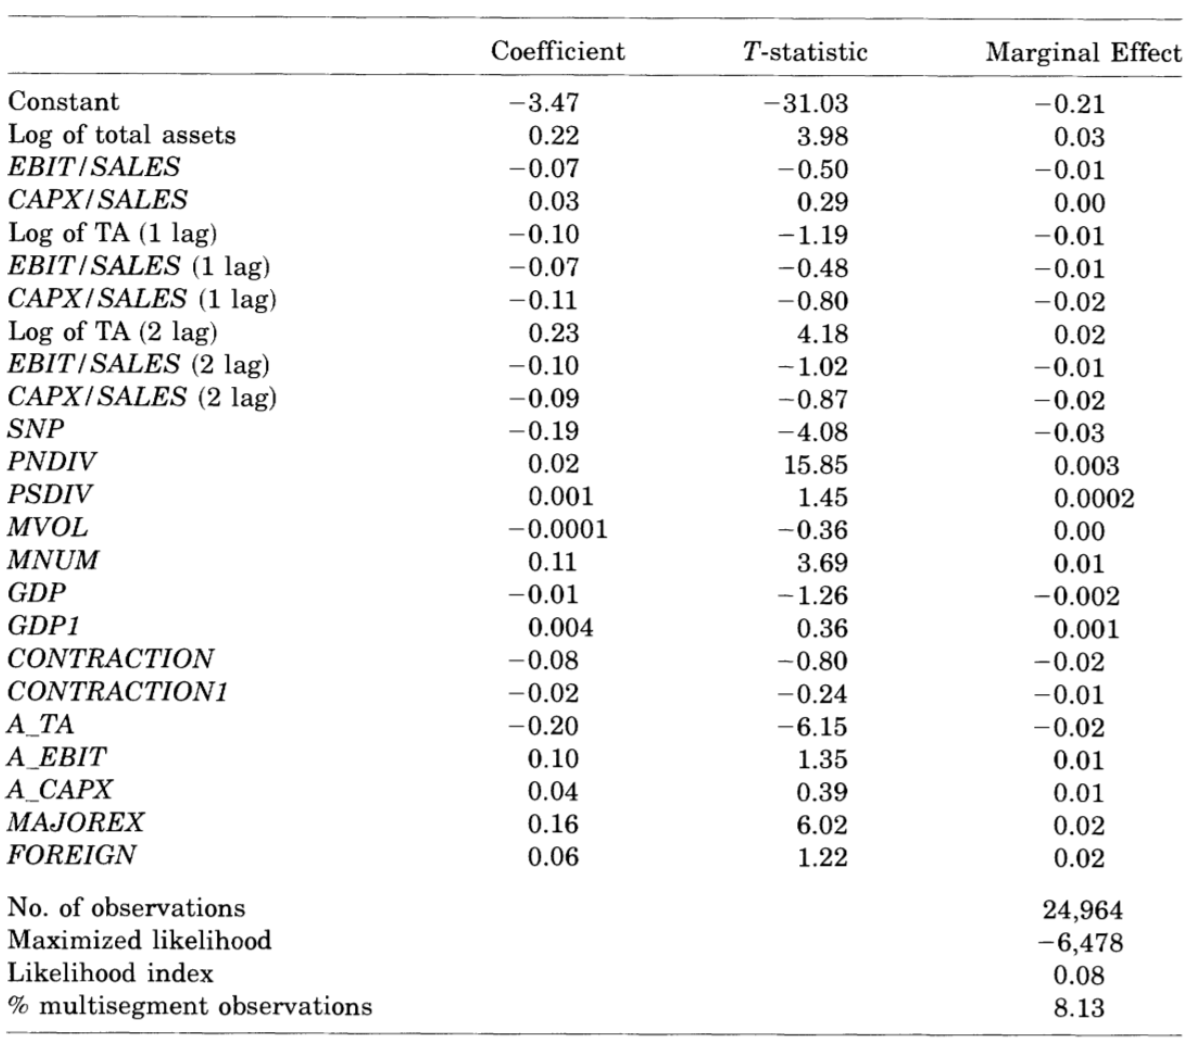
\includegraphics[width=0.6\linewidth]{figures/table8.png}
        \caption{}
    \end{figure}
\end{frame}

\begin{frame}{For refocusing firms}
    \begin{figure}
        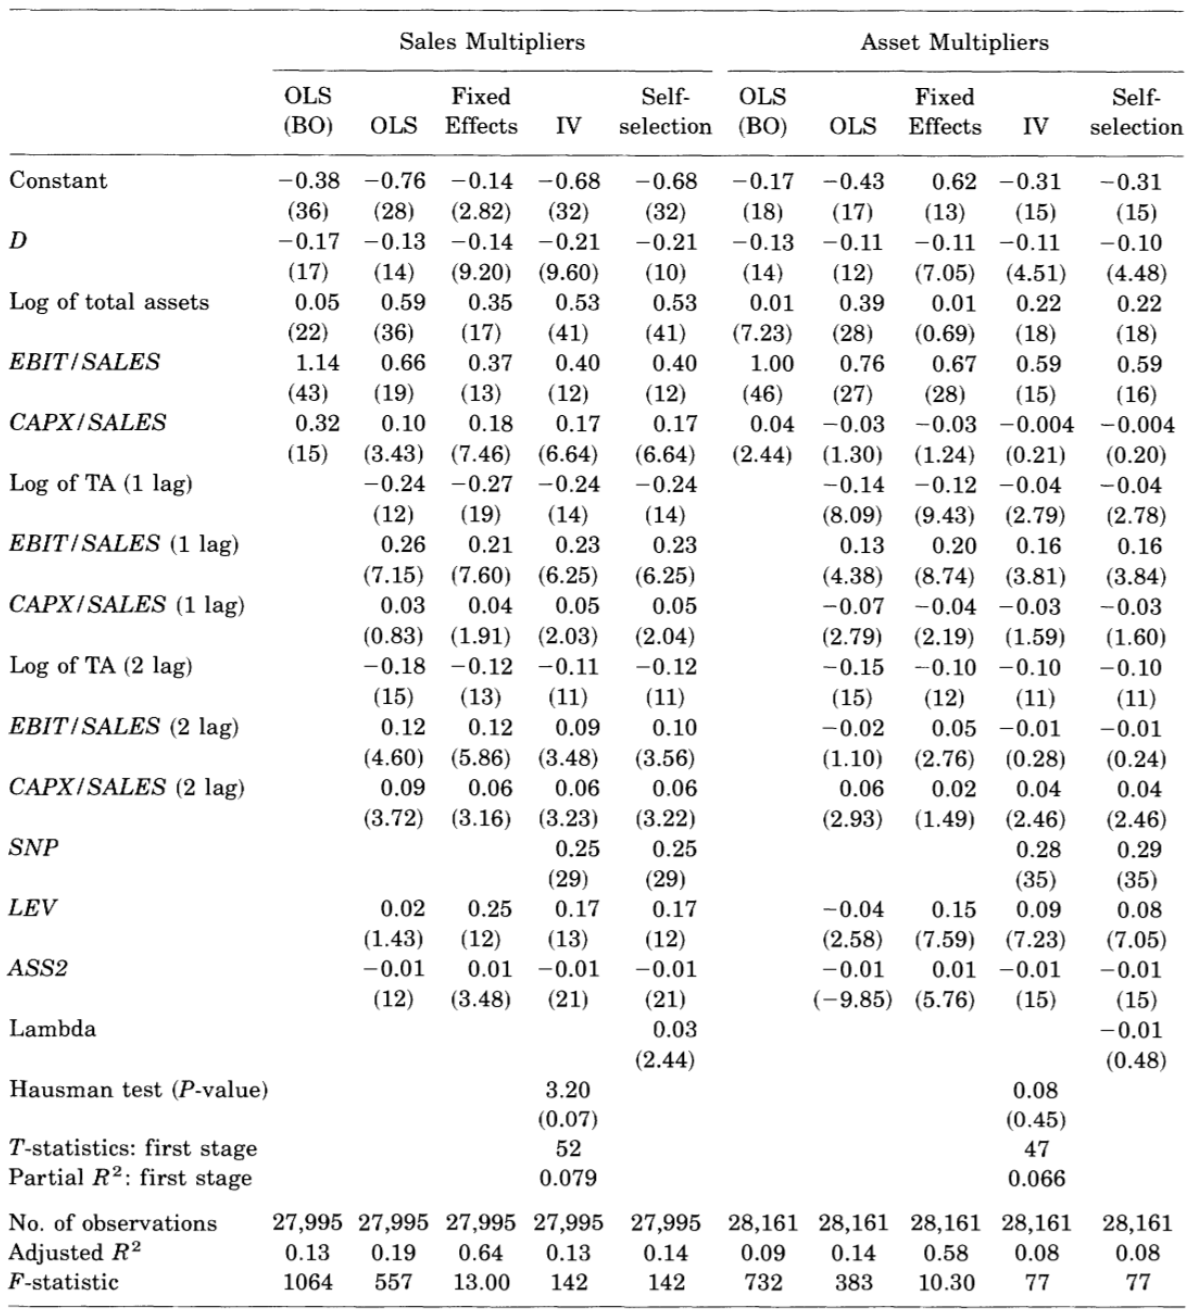
\includegraphics[width=0.5\linewidth]{figures/table9.png}
        \caption{}
    \end{figure}
\end{frame}

\begin{frame}{Probit estimates for refocusing firms}
    \begin{figure}
        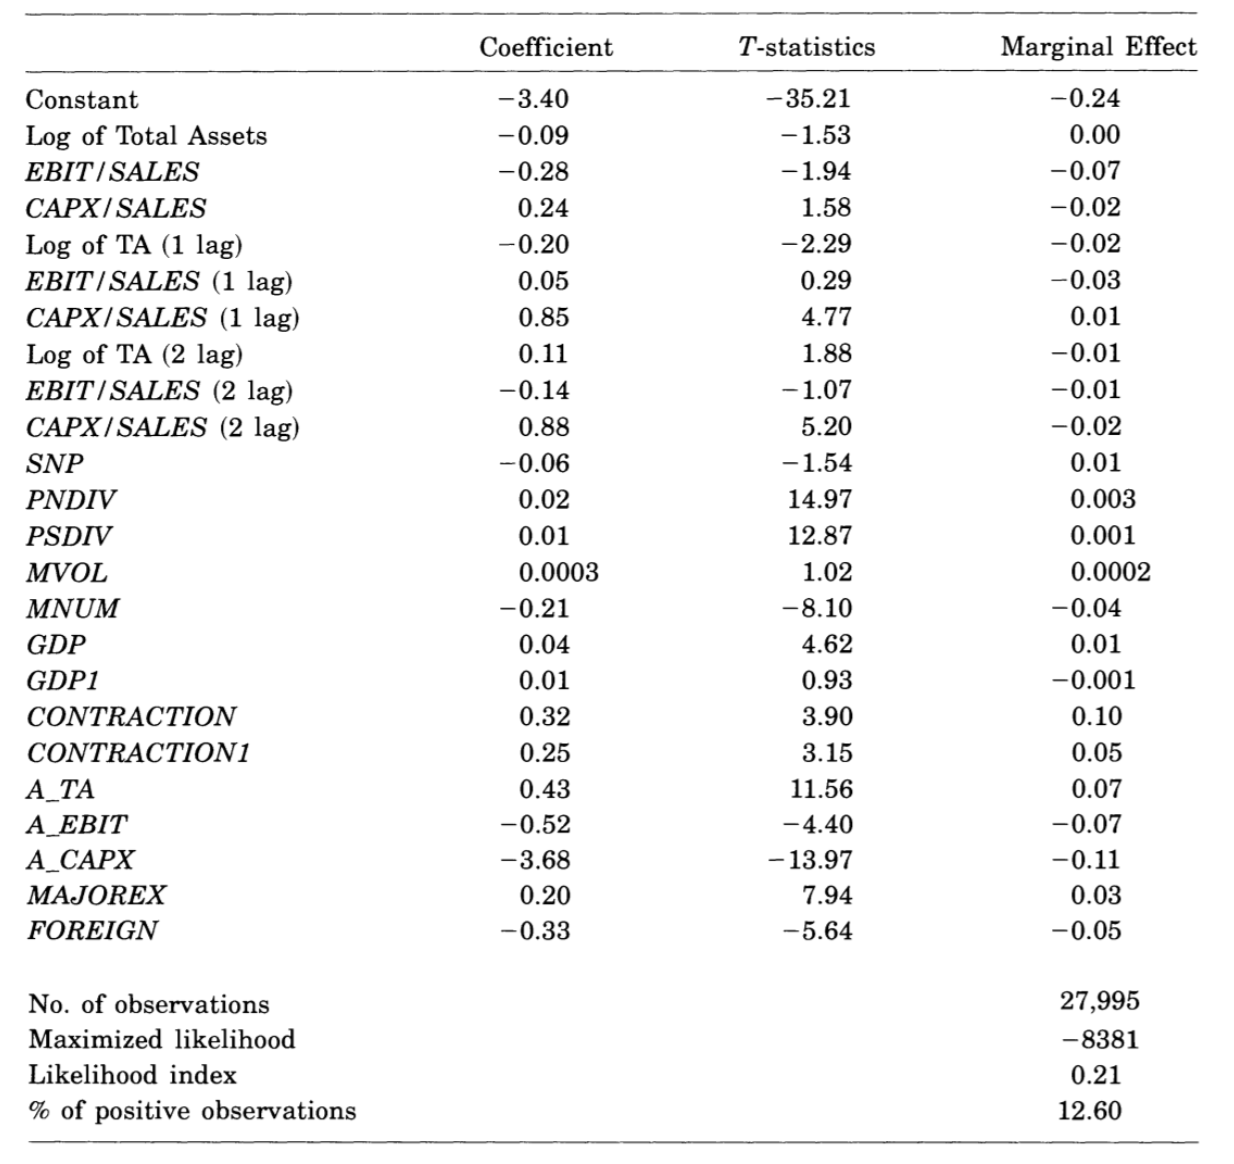
\includegraphics[width=0.6\linewidth]{figures/table10.png}
        \caption{}
    \end{figure}
\end{frame}

\section{Discussion}

\begin{frame}{From a investor's perspective}
    \begin{block}{Do investors like single segment firm better or conglomerates?}
        Investment portfolio vs business portfolio
    \end{block}
\end{frame}


\begin{frame}
    \Huge{\centerline{\textbf{The End}}}
\end{frame}

\end{document}